\documentclass[11pt, a4paper, twoside]{article}   	% use "amsart" instead of "article" for AMSLaTeX format

\usepackage{geometry}                		% See geometry.pdf to learn the layout options. There are lots.
\usepackage{pdfpages}
\usepackage{caption}
\usepackage{minted}
\usepackage[german]{babel}			% this end the next are needed for german umlaute
\usepackage[utf8]{inputenc}
\usepackage{color}
\usepackage{graphicx}
\usepackage{titlesec}
\usepackage{fancyhdr}
\usepackage{lastpage}
\usepackage{hyperref}
\usepackage[autostyle=false, style=english]{csquotes}
\usepackage{mathtools}
\usepackage{tabularx}
% http://www.artofproblemsolving.com/wiki/index.php/LaTeX:Symbols#Operators
% =============================================
% Layout & Colors
% =============================================
\geometry{
   a4paper,
   total={210mm,297mm},
   left=20mm,
   right=20mm,
   top=20mm,
   bottom=30mm
 }	

\definecolor{myred}{rgb}{0.8,0,0}
\definecolor{mygreen}{rgb}{0,0.6,0}
\definecolor{mygray}{rgb}{0.5,0.5,0.5}
\definecolor{mymauve}{rgb}{0.58,0,0.82}

\setcounter{secnumdepth}{4}


% the default java directory structure and the main packages
\newcommand{\srcDir}{../src/ImageJ/plugins/bva2}
\newcommand{\imageDir}{images}


% =============================================
% Code Settings
% =============================================
\newenvironment{code}{\captionsetup{type=listing}}{}
\newmintedfile[javaFile]{java}{
	linenos=true, 
	frame=single, 
	breaklines=true, 
	tabsize=2,
	numbersep=5pt,
	xleftmargin=10pt,
	baselinestretch=1,
	fontsize=\footnotesize
}

\newmintinline[inlineJava]{java}{}
\newminted[javaSource]{java}{
	breaklines=true, 
	tabsize=2,
	autogobble=true,
	breakautoindent=false
}


\newcommand{\xvdash}[1]{%
  \vdash^{\mkern-10mu\scriptscriptstyle\rule[-.9ex]{0pt}{0pt}#1}%
}

% =============================================
% Page Style, Footers & Headers, Title
% =============================================
\title{Übung 4}
\author{Gattringer Marko, Ruhsam Christoph}

\lhead{Gattringer Marko, Ruhsam Christoph}
\chead{BVA}
\rhead{Übung 4}

\lfoot{S1810454012, S1810454036}
\cfoot{}
\rfoot{ \thepage / \pageref{LastPage} }
\renewcommand{\footrulewidth}{0.4pt}
% =============================================
% D O C U M E N T     C O N T E N T
% =============================================
% =============================================
% 2016.10.13: 1 
% 2016.10.14: 2
% =============================================
\pagestyle{fancy}
\begin{document}
\setlength{\headheight}{15mm}
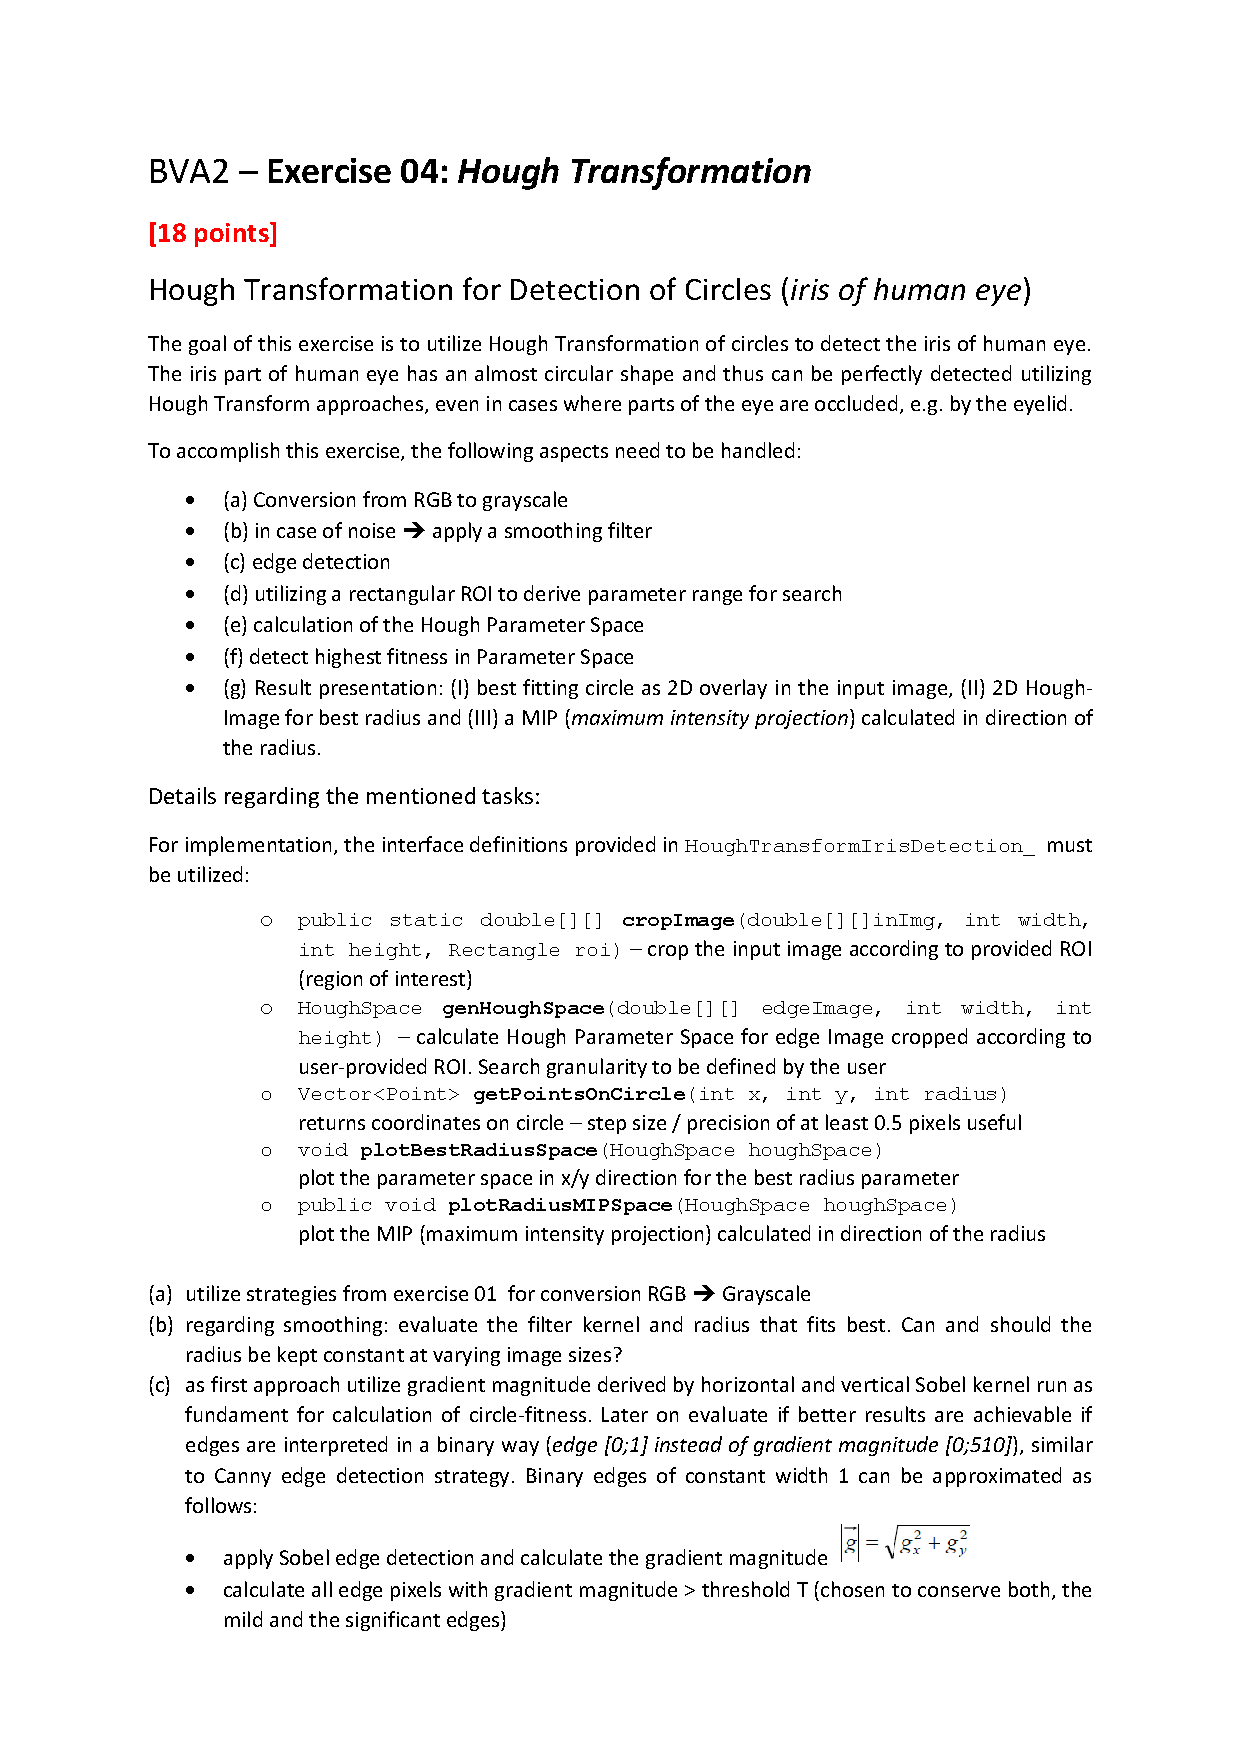
\includepdf[pages={1,2}]{Angabe.pdf}

\section{Hough Transformation}
\subsection{Lösungsidee}
\subsubsection{(a) Conversion from RGB to grayscale}
Diese Aufgabe wird mit der bereits in der Klasse \textit{ImageJUtility} implementierten Methode \textit{getGrayscaleImgFromRBG} gelöst. Jedoch wird die Implementierung um einen weiteren Case erweitert, in dem die gewichtete Berechnung, anstatt des Mittelwerts genommen wird. \newline \newline
\mbox{\LARGE $ grayValue = 0.299 * red + 0.587 * green + 0.114 * blue$}

\subsubsection{(b) in case of noise $\rightarrow$ apply a smoothing filter}
Diese Aufgabe wird mit der \textit{Anisotropen Diffusion} von Ruhsam Christoph der dritten Übung gelöst und wird hier nicht näher erläutert.
$\kappa = 20; iterations = 10$

\subsubsection{(c) edge detection}
Diese Aufgabe wird mit dem \textit{Sobel-Operator}, der gemeinsam in der Übung entwickelt wurde, gelöst. Dazu wird zuerst der SobelH auf das Bild nach der Anisotropen Diffusion angewandt. Danach der SobelV auf das Bild nach Anisotropen Diffusion. Diese beiden Bilder werden mit dem Satz des Pythagoras zu einem gemerged.

\subsubsection{(d) utilizing a rectangular ROI to derive parameter range for search}
Dieser Teil war bereits in dem Template vorhanden. Deshalb wird auch hier keine Lösungsidee angegeben.

\subsubsection{(e) calculation of the Hough Parameter Space}
Hier wird zuerst überprüft, ob es sich bei dem Bild um Hoch- oder Querformat handelt. Der \textbf{Radius} ergibt sich durch $min(width, height) / 2$.
Danach wird für jedes Pixel jeder Radius von $minRadius$ bis $radius$ durchlaufen. Hier wird für jeden Radius und jedes Grad von $0$ bis $360$ der \glqq Hit\grqq{} berechnet. Der x-Wert und y-Wert des Hit-Pixels ergibt sich durch: \newline \newline
\mbox{\LARGE $ xHit = Math.floor(x - rad * (Math.cos(t * Math.PI / 180)))$}\newline
\mbox{\LARGE $ yHit = Math.floor(y - rad * (Math.sin(t * Math.PI / 180)))$}\newline
\newline
, wobei $x$ und $y$ die Koordinaten des aktuellen Pixels sind, $rad$ der aktuelle Radius und $t$ das aktuelle Grad ist.
Sobald es einen Hit gibt, wird im HoughSpace an der Stelle \textbf{$hs.houghSpace[x][y][rad]$} der aktuelle Wert um $1$ inkrementiert.
 
\subsubsection{(f) detect highest fitness in Parameter Space}
Um den besten fitness-Wert zu finden, wird der gesamte HoughSpace durchlaufen und der max-Wert an der Stelle \textbf{$hs.houghSpace[x][y][rad]$} gesucht.

\subsubsection{(g) Result presentation}
Aufgrund dieser beiden Plots kann bereits die Qualität des Endergebnisses vorausgesagt werden. Jeder Hotspot (weiße Punkte) ist mit großer Wahrscheinlichkeit das Zentrum eines gefundenen Kreises. Je klarer und eindeutiger diese Hotspots sind, desto höher ist die Wahrscheinlichkeit das ein Kreis gefunden wurde und desto besser ist das Endergebnis (Vergleiche die jeweiligen Bilder der einzelnen Testfälle). 

\newpage
\subsection{Code}
\begin{code}
	\caption{HoughTransformIrisDetection\_.java}
	\javaFile{\srcDir/HoughTransformIrisDetection_.java}
	\label{src:HoughTransformIrisDetection_}
\end{code}

\newpage
\subsection{Tests und Auswertung}
\label{TestsUndAuswertung}
\subsubsection{Iris 4}
\begin{figure}[H]
	\centering
	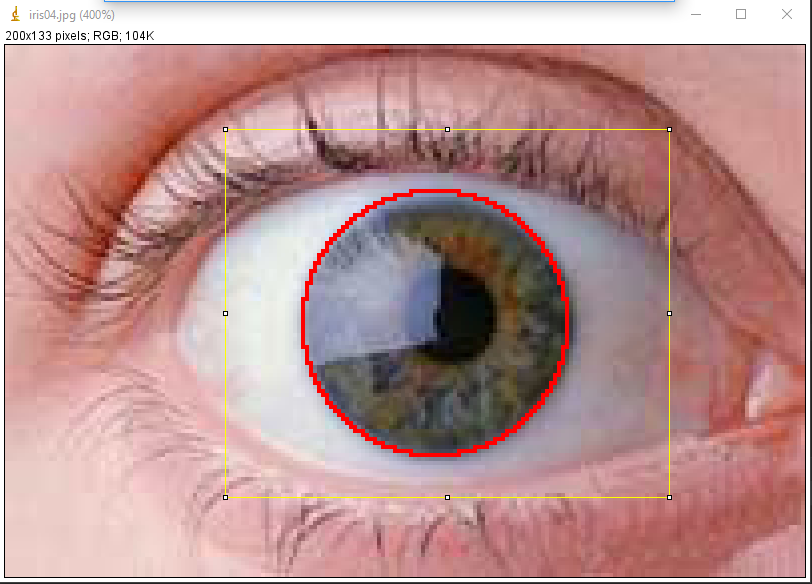
\includegraphics[scale=0.6]{\imageDir/Iris4detected.png}
	\caption{Original Image (detected iris)}
\end{figure}

\begin{figure}[H]
	\centering
	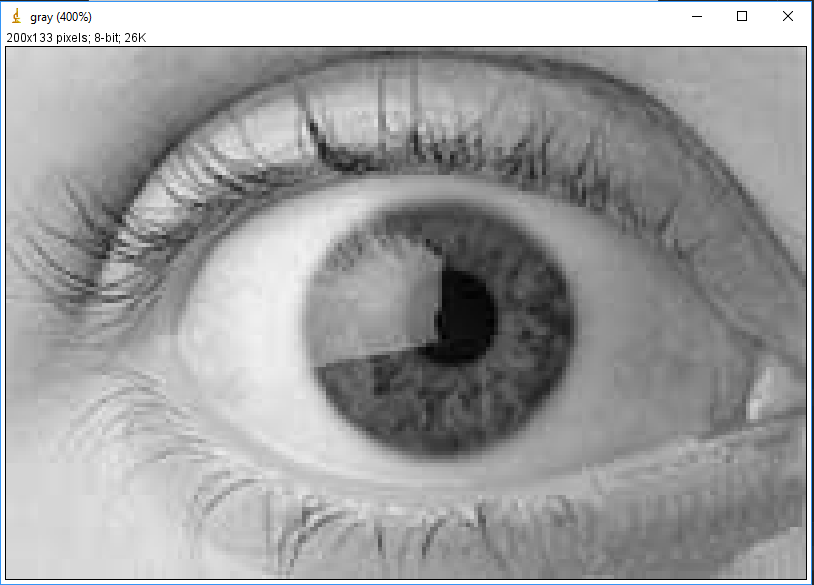
\includegraphics[scale=0.6]{\imageDir/Iris4gray.png}
	\caption{Gray Image after Conversion}
\end{figure}

\begin{figure}[H]
	\centering
	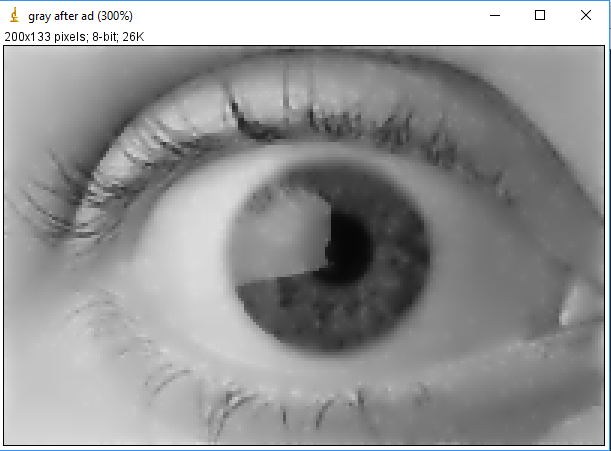
\includegraphics[scale=0.6]{\imageDir/Iris4grayafterAD.png}
	\caption{Gray Image after Conversion and Anisotropic Diffusion}
\end{figure}

\begin{figure}[H]
	\centering
	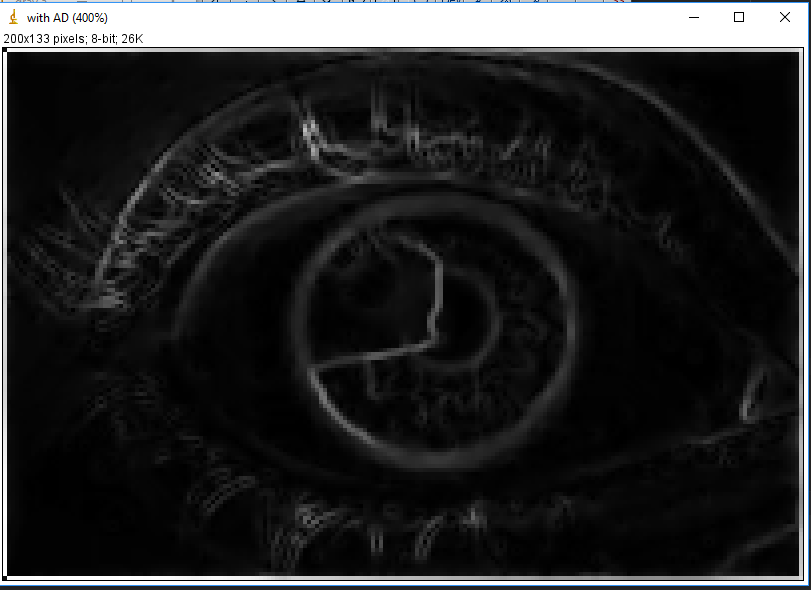
\includegraphics[scale=0.6]{\imageDir/Iris4aftersobel.png}
	\caption{Image after Sobel}
\end{figure}

\begin{figure}[H]
	\centering
	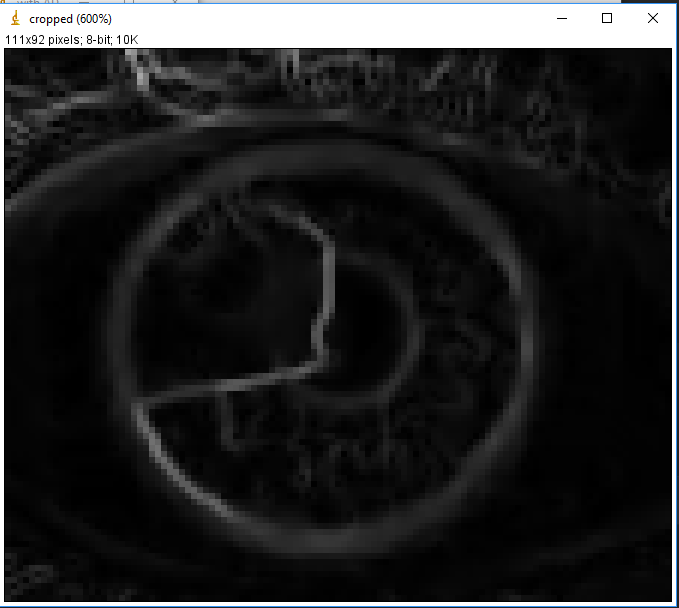
\includegraphics[scale=0.6]{\imageDir/Iris4cropped.png}
	\caption{Cropped Image}
\end{figure}

\begin{figure}[H]
	\centering
	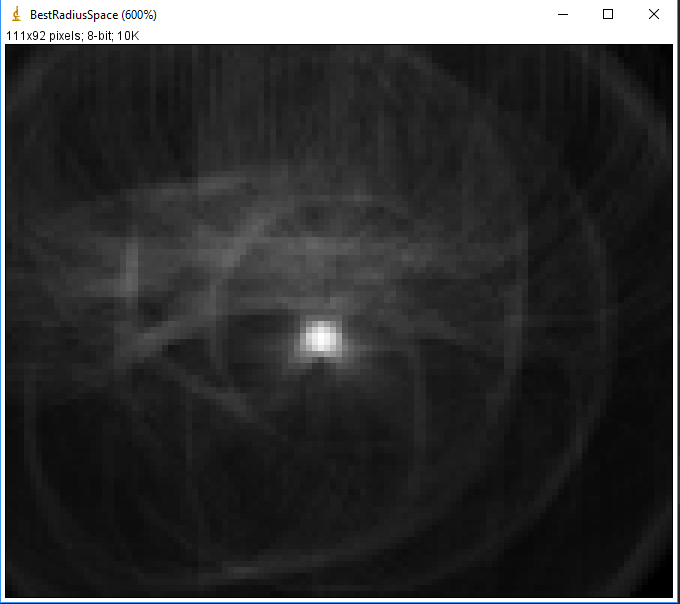
\includegraphics[scale=0.6]{\imageDir/Iris4BestRadiusSpace.png}
	\caption{Best Radius Space}
\end{figure}

\begin{figure}[H]
	\centering
	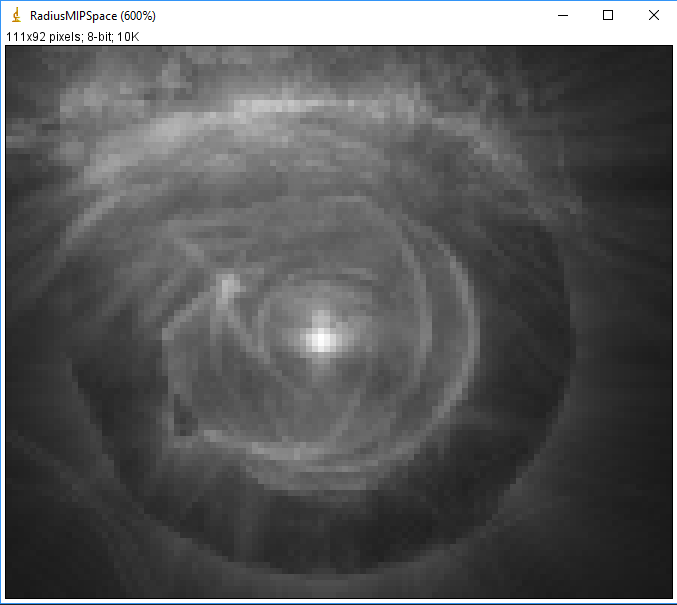
\includegraphics[scale=0.6]{\imageDir/Iris4RadiusMIPSpace.png}
	\caption{Radius MIP Space}
\end{figure}

\newpage
\subsubsection{Iris 5}
\begin{figure}[H]
	\centering
	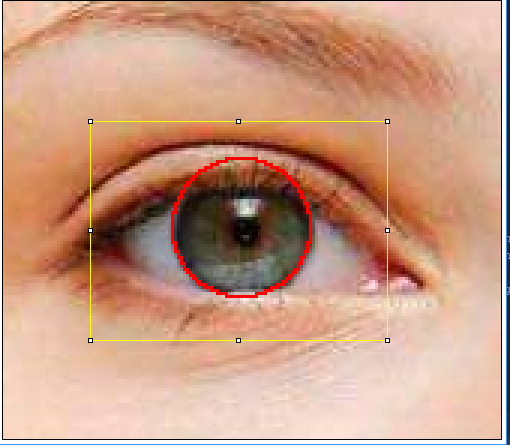
\includegraphics[scale=0.6]{\imageDir/Iris5detected.png}
	\caption{Original Image (detected iris)}
\end{figure}

\begin{figure}[H]
	\centering
	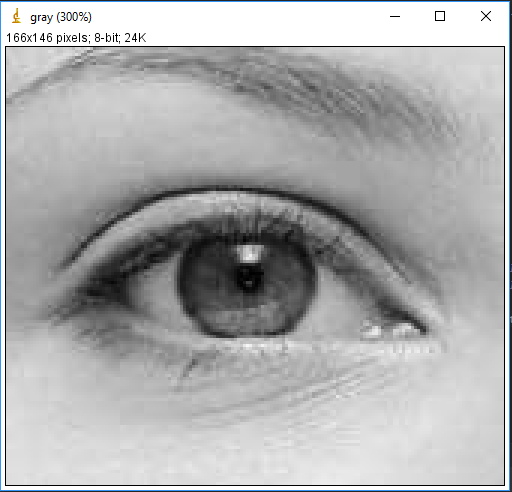
\includegraphics[scale=0.6]{\imageDir/Iris5gray.png}
	\caption{Gray Image after Conversion}
\end{figure}

\begin{figure}[H]
	\centering
	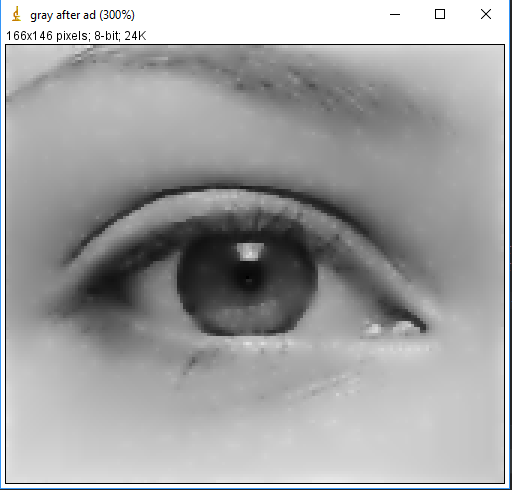
\includegraphics[scale=0.6]{\imageDir/Iris5grayafterAD.png}
	\caption{Gray Image after Conversion and Anisotropic Diffusion}
\end{figure}

\begin{figure}[H]
	\centering
	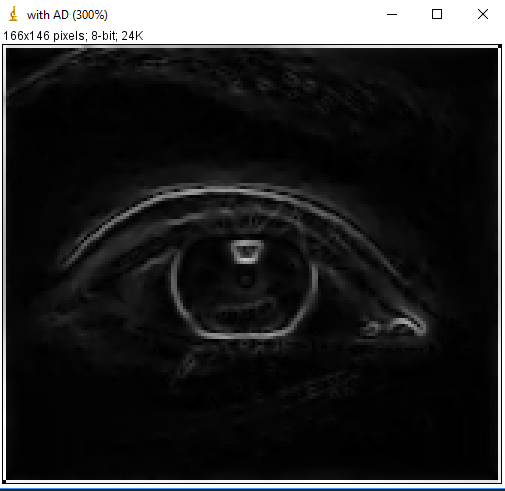
\includegraphics[scale=0.6]{\imageDir/Iris5aftersobel.png}
	\caption{Image after Sobel}
\end{figure}

\begin{figure}[H]
	\centering
	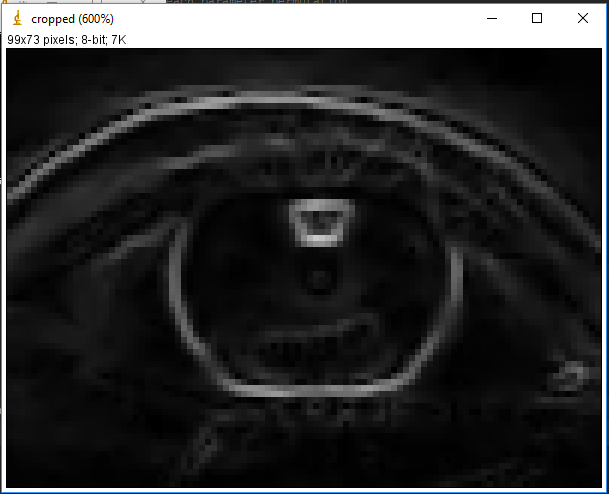
\includegraphics[scale=0.6]{\imageDir/Iris5cropped.png}
	\caption{Cropped Image}
\end{figure}

\begin{figure}[H]
	\centering
	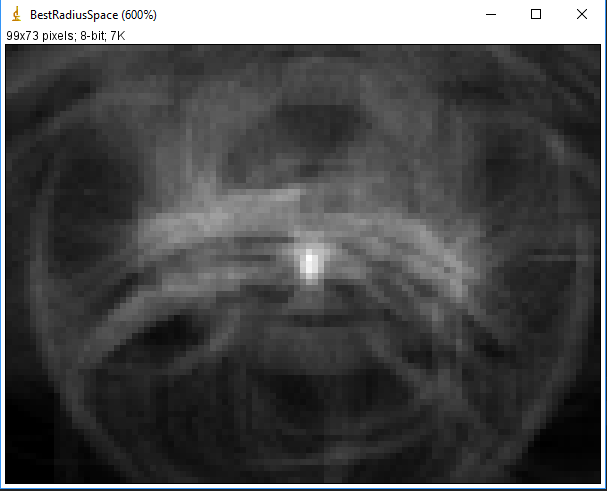
\includegraphics[scale=0.6]{\imageDir/Iris5BestRadiusSpace.png}
	\caption{Best Radius Space}
	\label{fig-best-radius-iris5}
\end{figure}

\begin{figure}[H]
	\centering
	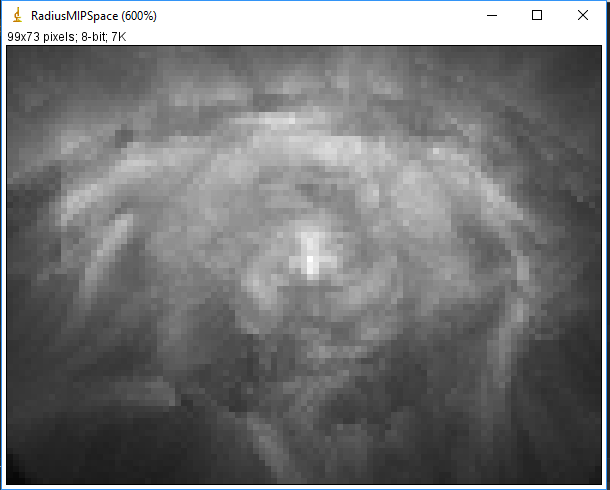
\includegraphics[scale=0.6]{\imageDir/Iris5RadiusMIPSpace.png}
	\caption{Radius MIP Space}
	\label{fig-mip-space-iris5}
\end{figure}

\newpage
\subsubsection{Iris 6}
\begin{figure}[H]
	\centering
	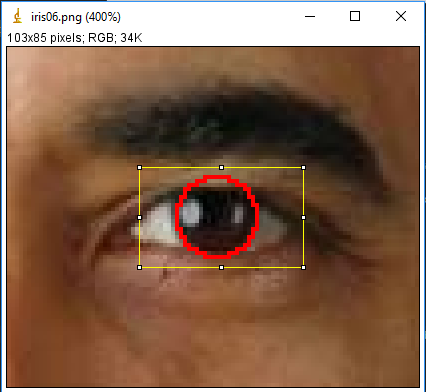
\includegraphics[scale=0.6]{\imageDir/Iris6detected.png}
	\caption{Original Image (detected iris)}
\end{figure}

\begin{figure}[H]
	\centering
	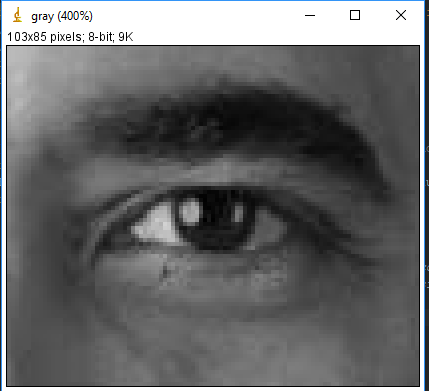
\includegraphics[scale=0.6]{\imageDir/Iris6gray.png}
	\caption{Gray Image after Conversion}
\end{figure}

\begin{figure}[H]
	\centering
	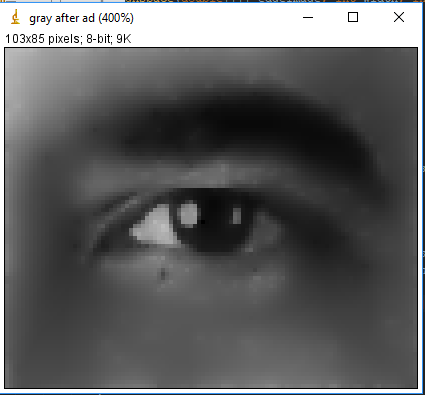
\includegraphics[scale=0.6]{\imageDir/Iris6grayafterAD.png}
	\caption{Gray Image after Conversion and Anisotropic Diffusion}
\end{figure}

\begin{figure}[H]
	\centering
	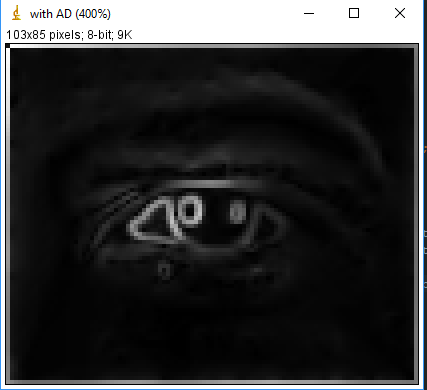
\includegraphics[scale=0.6]{\imageDir/Iris6aftersobel.png}
	\caption{Image after Sobel}
\end{figure}

\begin{figure}[H]
	\centering
	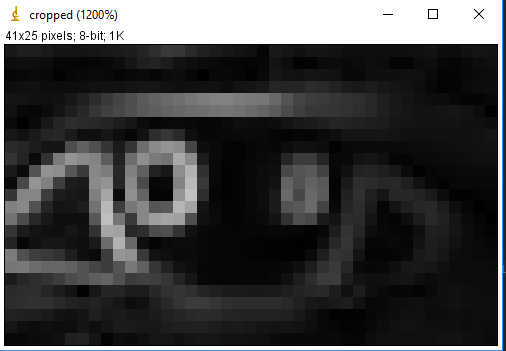
\includegraphics[scale=0.6]{\imageDir/Iris6cropped.png}
	\caption{Cropped Image}
\end{figure}

\begin{figure}[H]
	\centering
	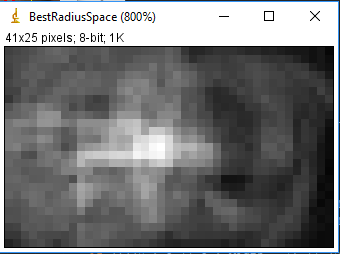
\includegraphics[scale=0.6]{\imageDir/Iris6BestRadiusSpace.png}
	\caption{Best Radius Space}
\end{figure}

\begin{figure}[H]
	\centering
	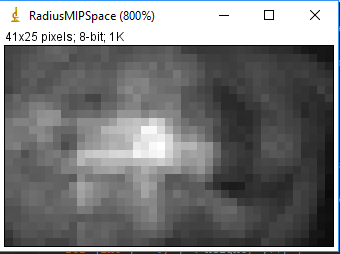
\includegraphics[scale=0.6]{\imageDir/Iris6RadiusMIPSpace.png}
	\caption{Radius MIP Space}
\end{figure}

\end{document}